\section{LQR}
\subsection{Simulink}

Figure~\ref{fig:LQR simulink} contains the Simulink diagram, which contains a subsystem instead of the simulink discrete statespace. This is because the states are used by the controller, the subsystem is displayed in figure~\ref{fig:LQR simulink subsystem}. The feedback law given in the assignment :$u(k)=u_{ref}(k) - K ( x(k)-x_{ref}(k) )$ is applied. A Saturation block is placed before the linear system to clip the control actions.

\begin{figure}[H]
	\centering
	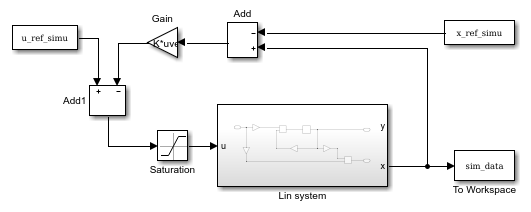
\includegraphics[width=\textwidth]{./LQR/not_generated/LQR_simulink.png}
	\caption{LQR in simulink}
	\label{fig:LQR simulink}
\end{figure}

\begin{figure}[H]
	\centering
	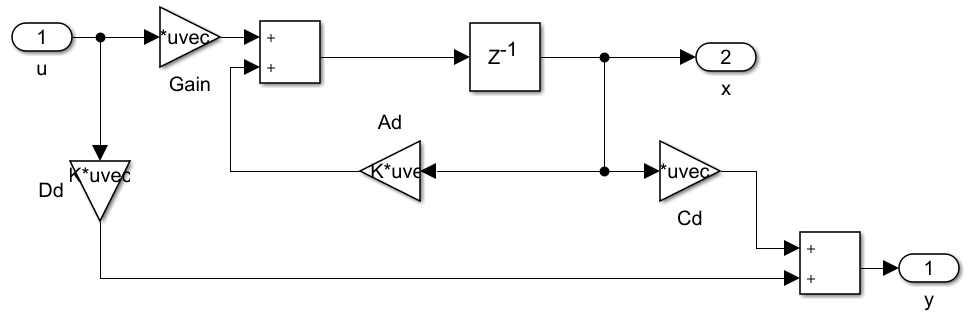
\includegraphics[width=0.6\textwidth]{./LQR/not_generated/simulink_subsys.png}
	\caption{LQR in simulink}
	\label{fig:LQR simulink subsystem}
\end{figure}

\subsection{Numerical values gain matrices LQR1 and LQR2}
The assignment specifically asked for the numerical values of the gains:

$$
K_{LQR_1} = 
\begin{bmatrix}
88.37 & 0 & 0 & 135.87 & 0 & 0 \\
0 & 88.37 & 0 & 0 & 135.87 & 0 \\
0 & 0 & 11.01 & 0 & 0 & 12.68 \\
\end{bmatrix}
$$

$$
K_{LQR_2} = 
\begin{bmatrix}
90.82 & 0 & 0 & 110.19 & 0 & 0 \\
0 & 90.82 & 0 & 0 & 110.2 & 0 \\
0 & 0 & 46.26 & 0 & 0 & 12.90 \\
\end{bmatrix}
$$

\subsection{Simulation results LQR1 and LQR2}

The assignment states the matrix $R=10^{-4} I_{3x3}$ for $LQR_1$ and $LQR_2$ , $Q=I_{6x6}$ for $LQR_1$ and $Q=diag(1,1,1,0,0,0)$ for $LQR_2$.

\begin{equation}
	J=x^TQx + u^TRu
\end{equation}

The trajectories followed by $LQR_1$ are about the same as $LQR_2$ this is visible on  figure~\ref{fig:simulink simulations LQR1 and LQR2 - trajects}. The inputs are also about the same this is visible on figure~\ref{fig:simulink simulations LQR1 and LQR2 - inputs}. This is not surprising at all as the keeper was already taking very smooth corners, reducing the weights on the speed $v_X$, $v_y$ and $v_{\omega}$ will reduce over-steering. 

%Except for the very severe over steering at the sharpest corner, there is nearly no over steering in this case. The very bad over steering is due to clipping on the inputs, figure~\ref{fig:least square opti simulation, better condition} very clearly has an to large input at the start and near the end of the trajectory. There is little difference between the two controllers. 

Figure~\ref{fig:trajectory LQR1 and LQR2 on 1 graph} contains both trajectory's on one graph, the bottom part of the picture is zoomed in on the corner where there is a slight difference. Here its visible that LQR2 does not optimize optimize on speed which makes it over steer a bit more in that corner. 

Figure~\ref{fig:simulink simulations LQR1 and LQR2 - inputs} clearly shows inputs on $F_x$ and $F_y$ that are clipped as they are suddenly flat at the maximum value. This obviously is a problem and explains why the keeper is not following the reference near the end and the start of the path on figure~\ref{fig:simulink simulations LQR1 and LQR2 - trajects}. 

\begin{figure}[H]
	\centering
	\begin{subfigure}[b]{0.45\textwidth}
		\includegraphics[width=\textwidth]{./LQR/LQR1_traject.png}
		\caption{$LQR_1$ trajectory}
		\label{fig:LQR1 traject}
	\end{subfigure}
	\begin{subfigure}[b]{0.45\textwidth}
		\includegraphics[width=\textwidth]{./LQR/LQR2_traject.png}
		\caption{$LQR_2$ trajectory}
		\label{fig:LQR2 traject}
	\end{subfigure}
	\begin{subfigure}[b]{0.55\textwidth}
		\includegraphics[width=\textwidth]{./LQR/LQR_compare.png}
		\caption{trajectory LQR1 and LQR2 on 1 graph}
		\label{fig:trajectory LQR1 and LQR2 on 1 graph}
	\end{subfigure}
	\caption{simulations with the controller in Simulink with $u_{ref}$ and $x_{ref}$}
	\label{fig:simulink simulations LQR1 and LQR2 - trajects}
\end{figure}


\begin{figure}[H]
	\centering
	\begin{subfigure}[b]{0.45\textwidth}
		\includegraphics[width=\textwidth]{./LQR/LQR1_input.png}
		\caption{$LQR_1$ input}
		\label{fig:LQR1 input}
	\end{subfigure}
	\begin{subfigure}[b]{0.45\textwidth}
		\includegraphics[width=\textwidth]{./LQR/LQR2_input.png}
		\caption{$LQR_2$ input}
		\label{fig:LQR2 input}
	\end{subfigure}
	\caption{input data of the simulations with the controller in simulink with $u_{ref}$ and $x_{ref}$}
	\label{fig:simulink simulations LQR1 and LQR2 - inputs}
\end{figure}


%\begin{figure}[H]
%	\centering
%	\begin{subfigure}[b]{0.45\textwidth}
%		\includegraphics[width=\textwidth]{./LQR/LQRincreasedR_traject.png}
%		\caption{$LQR_3$ traject}
%		\label{fig:LQR3 traject}
%	\end{subfigure}
%	\begin{subfigure}[b]{0.45\textwidth}
%		\includegraphics[width=\textwidth]{./LQR/LQRincreasedR_input.png}
%		\caption{$LQR_3$ input}
%		\label{fig:LQR3 input}
%	\end{subfigure}
%	\caption{input data of the simulations with the controller in simulink with $u_{ref}$ and $x_{ref}$ Q is increased to $10^{-1}$}
%	\label{fig:simulink simulations LQR1 and LQR2 - increased Q}
%\end{figure}

\subsection{The total simulation cost for each controller}
The LQR controller tries to minimize the  objective function $J = x^TQx + u^TRu$. Table~\ref{tab:total-simulation cost LQR} contains the actual values of the objective function. $LQR_2$ did not follow the reference path as close at $LQR_1$ and has an objective function that is about 0.01\% higher. The figures already showed that the difference was insignificant. Obviously its very hard to make any kind of concussions solely based on these figures.

\begin{minipage}{\linewidth}
	\centering
	\captionof{table}{total-simulation cost $LQR_1$, $LQR_2$} 
	\label{tab:total-simulation cost LQR} 
	\begin{tiny}\begin{tabular}{|c|c|}
\hline
\textbf{$LQR_1$}&\textbf{$LQR_2$}\\\hline
3.7231e+04&3.7236e+04\\\hline
\end{tabular}
\end{tiny}
\end{minipage}
